%%% main document {{{

\documentclass[
a4paper,     %% defines the paper size: a4paper (default), a5paper, letterpaper, ...
% landscape,   %% sets the orientation to landscape
% twoside,     %% changes to a two-page-layout (alternatively: oneside)
% twocolumn,   %% changes to a two-column-layout
% headsepline, %% add a horizontal line below the column title
% footsepline, %% add a horizontal line above the page footer
% titlepage,   %% only the titlepage (using titlepage-environment) appears on the first page (alternatively: notitlepage)
% parskip,     %% insert an empty line between two paragraphs (alternatively: halfparskip, ...)
% leqno,       %% equation numbers left (instead of right)
% fleqn,       %% equation left-justified (instead of centered)
% tablecaptionabove, %% captions of tables are above the tables (alternatively: tablecaptionbelow)
% draft,       %% produce only a draft version (mark lines that need manual edition and don't show graphics)
% 10pt         %% set default font size to 10 point
% 11pt         %% set default font size to 11 point
12pt         %% set default font size to 12 point
]{scrartcl}  %% article, see KOMA documentation (scrguide.dvi)



%%%%%%%%%%%%%%%%%%%%%%%%%%%%%%%%%%%%%%%%%%%%%%%%%%%%%%%%%%%%%%%%%%%%%%%%%%%%%%%%
%%%
%%% packages
%%%

%%%
%%% encoding and language set
%%%

%%% ngerman: language set to new-german
%\usepackage{english}

%%% babel: language set (can cause some conflicts with package ngerman)
%%%        use it only for multi-language documents or non-german ones
\usepackage[english]{babel}

%%% inputenc: coding of german special characters
\usepackage[utf8]{inputenc}

%%% fontenc, ae, aecompl: coding of characters in PDF documents
\usepackage[T1]{fontenc}
\usepackage{ae,aecompl}

\usepackage{caption}
\usepackage{subcaption}

%%%
%%% technical packages
%%%

%%% amsmath, amssymb, amstext: support for mathematics
\usepackage{amsmath,amssymb,amstext}

%%% psfrag: replace PostScript fonts
\usepackage{psfrag}

%%% listings: include programming code
\usepackage{listings}

%%% units: technical units
%\usepackage{units}

%%%
%%% layout
%%%

%%% scrpage2: KOMA heading and footer
%%% Note: if you don't use this package, please remove 
%%%       \pagestyle{scrheadings} and corresponding settings
%%%       below too.
\usepackage[automark]{scrpage2}

\usepackage{wrapfig}

\usepackage{paralist}


%%%
%%% PDF
%%%

\usepackage{ifpdf}

%%% Should be LAST usepackage-call!
%%% For docu on that, see reference on package ``hyperref''
\ifpdf%   (definitions for using pdflatex instead of latex)

  %%% graphicx: support for graphics
  \usepackage[pdftex]{graphicx}

  \pdfcompresslevel=9

  %%% hyperref (hyperlinks in PDF): for more options or more detailed
  %%%          explanations, see the documentation of the hyperref-package
  \usepackage[%
    %%% general options
    pdftex=true,      %% sets up hyperref for use with the pdftex program
    %plainpages=false, %% set it to false, if pdflatex complains: ``destination with same identifier already exists''
    %
    %%% extension options
    backref,      %% adds a backlink text to the end of each item in the bibliography
    pagebackref=false, %% if true, creates backward references as a list of page numbers in the bibliography
    colorlinks=true,   %% turn on colored links (true is better for on-screen reading, false is better for printout versions)
    %
    %%% PDF-specific display options
    bookmarks=true,          %% if true, generate PDF bookmarks (requires two passes of pdflatex)
    bookmarksopen=false,     %% if true, show all PDF bookmarks expanded
    bookmarksnumbered=false, %% if true, add the section numbers to the bookmarks
    %pdfstartpage={1},        %% determines, on which page the PDF file is opened
    pdfpagemode=None         %% None, UseOutlines (=show bookmarks), UseThumbs (show thumbnails), FullScreen
  ]{hyperref}


  %%% provide all graphics (also) in this format, so you don't have
  %%% to add the file extensions to the \includegraphics-command
  %%% and/or you don't have to distinguish between generating
  %%% dvi/ps (through latex) and pdf (through pdflatex)
  \DeclareGraphicsExtensions{.pdf}

\else %else   (definitions for using latex instead of pdflatex)

  \usepackage[dvips]{graphicx}

  \DeclareGraphicsExtensions{.eps}

  \usepackage[%
    dvips,           %% sets up hyperref for use with the dvips driver
    colorlinks=false %% better for printout version; almost every hyperref-extension is eliminated by using dvips
  ]{hyperref}

\fi


%%% sets the PDF-Information options
%%% (see fields in Acrobat Reader: ``File -> Document properties -> Summary'')
%%% Note: this method is better than as options of the hyperref-package (options are expanded correctly)
\hypersetup{
  pdftitle={Image Processing and Pattern Recognition}, %%
  pdfauthor={Christian Ertler (1030970), Peter Prodinger (0430935)}, %%
  pdfsubject={Visual Sudoku Solver}, %%
  pdfcreator={Accomplished with LaTeX2e and pdfLaTeX with hyperref-package.}, %% 
  pdfproducer={}, %%
  pdfkeywords={} %%
}


%%%%%%%%%%%%%%%%%%%%%%%%%%%%%%%%%%%%%%%%%%%%%%%%%%%%%%%%%%%%%%%%%%%%%%%%%%%%%%%%
%%%
%%% user defined commands
%%%

%%% \mygraphics{}{}{}
%% usage:   \mygraphics{width}{filename_without_extension}{caption}
%% example: \mygraphics{0.7\textwidth}{rolling_grandma}{This is my grandmother on inlinescates}
%% requires: package graphicx
%% provides: including centered pictures/graphics with a boldfaced caption below
%% 
\newcommand{\mygraphics}[3]{
  \begin{center}
    \includegraphics[width=#1, keepaspectratio=true]{#2} \\
    \textbf{#3}
  \end{center}
}

%%%%%%%%%%%%%%%%%%%%%%%%%%%%%%%%%%%%%%%%%%%%%%%%%%%%%%%%%%%%%%%%%%%%%%%%%%%%%%%%
%%%
%%% define the titlepage
%%%

\subject{Visual Sudoku Solver}   %% subject which appears above titlehead
% \titlehead{} %% special heading for the titlepage

%%% title
\title{Image Processing and Pattern Recognition}

%%% author(s)
\author{Christian Ertler (1030970) \\ Peter Prodinger (0430935)}

%%% date
\date{Graz, \today{}}

% \publishers{}

% \thanks{} %% use it instead of footnotes (only on titlepage)

% \dedication{} %% generates a dedication-page after titlepage


%%% uncomment following lines, if you want to:
%%% reuse the maketitle-entries for hyperref-setup
%\newcommand\org@maketitle{}
%\let\org@maketitle\maketitle
%\def\maketitle{%
%  \hypersetup{
%    pdftitle={\@title},
%    pdfauthor={\@author}
%    pdfsubject={\@subject}
%  }%
%  \org@maketitle
%}


%%%%%%%%%%%%%%%%%%%%%%%%%%%%%%%%%%%%%%%%%%%%%%%%%%%%%%%%%%%%%%%%%%%%%%%%%%%%%%%%
%%%
%%% set heading and footer
%%%

%%% scrheadings default: 
%%%      footer - middle: page number
\pagestyle{scrheadings}

%%% user specific
%%% usage:
%%% \position[heading/footer for the titlepage]{heading/footer for the rest of the document}

%%% heading - left
% \ihead[]{}

%%% heading - center
% \chead[]{}

%%% heading - right
% \ohead[]{}

%%% footer - left
% \ifoot[]{}

%%% footer - center
% \cfoot[]{}

%%% footer - right
% \ofoot[]{}



%%%%%%%%%%%%%%%%%%%%%%%%%%%%%%%%%%%%%%%%%%%%%%%%%%%%%%%%%%%%%%%%%%%%%%%%%%%%%%%%
%%%
%%% begin document
%%%

\setlength{\parindent}{0cm}

\begin{document}

\maketitle

% \pagenumbering{roman} %% small roman page numbers

%%% include the title
% \thispagestyle{empty}  %% no header/footer (only) on this page

%%% start a new page and display the table of contents
% \newpage
% \tableofcontents

%%% start a new page and display the list of figures
% \newpage
% \listoffigures

%%% start a new page and display the list of tables
% \newpage
% \listoftables

%%% display the main document on a new page 
% \newpage

% \pagenumbering{arabic} %% normal page numbers (include it, if roman was used above)

%%%%%%%%%%%%%%%%%%%%%%%%%%%%%%%%%%%%%%%%%%%%%%%%%%%%%%%%%%%%%%%%%%%%%%%%%%%%%%%%
%%%
%%% begin main document
%%% structure: \section \subsection \subsubsection \paragraph \subparagraph
%%%

%%%%%%%%%%%%%%%%%%%%%%%%%%%%%
\section{Introduction}
%%%%%%%%%%%%%%%%%%%%%%%%%%%%%

The goal of this project was to implement a visual sudoku solver which should be able
to locate a sudoku field in a video taken from a webcam and present the solution of it
directly on the empty cells in the original image. The application should run in realtime
and be capable of solving arbitrary sudokus. 

% \begin{figure}
%     \centering
%     \begin{subfigure}[b]{0.45\textwidth}
%         \centering
%         \includegraphics[width=\textwidth]{results/1_elefant_bw.jpg}
%         \caption{Original image}
%     \end{subfigure}
%     \begin{subfigure}[b]{0.45\textwidth}
%         \centering
%         \includegraphics[width=\textwidth]{results/1_elefant_bw_e.jpg}
%         \caption{Contrast enhanced image}
%     \end{subfigure}

%     \begin{subfigure}[b]{0.30\textwidth}
%         \centering
%         \includegraphics[width=\textwidth]{results/1_elefant_bw_ohist.jpg}
%         \caption{Original histogram}
%     \end{subfigure}
%     \begin{subfigure}[b]{0.30\textwidth}
%         \centering
%         \includegraphics[width=\textwidth]{results/1_elefant_bw_chist.jpg}
%         \caption{Cumulative histogram}
%     \end{subfigure}
%     \begin{subfigure}[b]{0.30\textwidth}
%         \centering
%         \includegraphics[width=\textwidth]{results/1_elefant_bw_ehist.jpg}
%         \caption{Equalized Histogram}
%     \end{subfigure}
%     \caption{elefant\_bw.jpg}
%     \label{fig:1_elefant_bw}
% \end{figure}



%%%%%%%%%%%%%%%%%%%%%%%%%%%%%
\section{Methods}
%%%%%%%%%%%%%%%%%%%%%%%%%%%%%

In this section we will describe the methods we used to reach our goals.

\subsection{Finding and preparing the sudoku field}
\label{sec:find}

First of all, the sudoku field must be localized and prepared for further
processing. By means of simplicity we assume that the sudoku field must be
the dominant object in the image. Furthermore, it must be clearly outlined by
an thick dark frame. Most of the sudokus in papers and magazines fulfill this
criteria.

To find the sudoku a contour based segmentation of the image preprocessed by
a Canny edge detector is done. A sample output of the Canny filter can be seen
in figure \ref{fig:canny}. Since a sudoku is always square or rectangular
it will appear as a quadrilateral in the image. Therefore, we can just take 
the biggest convex contour as the contour of the sudoku field.

\begin{figure}
    \centering
    \begin{subfigure}[b]{0.45\textwidth}
        \centering
        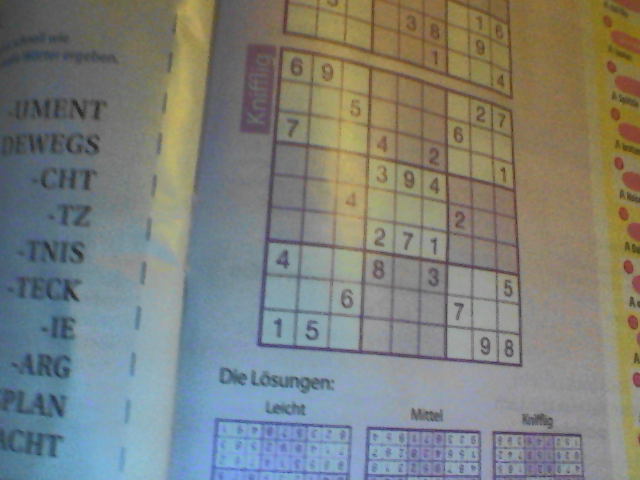
\includegraphics[width=\textwidth]{imgs/canny_frame.png}
        \caption{Original frame.}
    \end{subfigure}
    \begin{subfigure}[b]{0.45\textwidth}
        \centering
        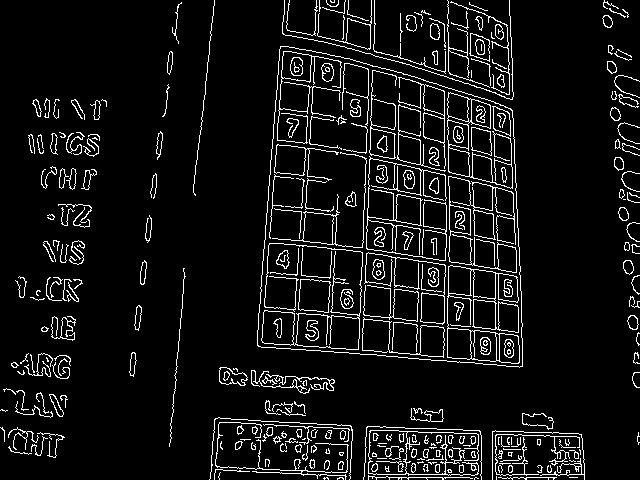
\includegraphics[width=\textwidth]{imgs/canny.png}
        \caption{Output of the canny filter.}
    \end{subfigure}
    \caption{Canny filtering}
    \label{fig:canny}
\end{figure}

Most of the time the sudoku will not be presented parallel to image plane so
it will be distorted perspectively. In order to simplify the further processing
we need to remove the perspective by finding a homography between the found
contour and a proper square. Since the contour consists of many points we need
to reduce it to the 4 corner points of the quadrilateral. For that purpose we
implemented an algorithm which approximates
the best fitting quadrilateral to a polygon\footnote{\url{http://stackoverflow.com/questions/2048024/minimum-area-quadrilateral-algorithm/2050478\#2050478}}.

We also tried to use a Hough-Transformation to find those points but the
other approach appeared to be more robust.

Having the corner points the homography can easily be computed and applied
to the image to perspectively unwarp the sudoku field. Additionally the field
is scaled to a fixed size to avoid scale issues. Figure \ref{fig:unwarping}
shows the unwarping.

\begin{figure}
    \centering
    \begin{subfigure}[b]{0.70\textwidth}
        \centering
        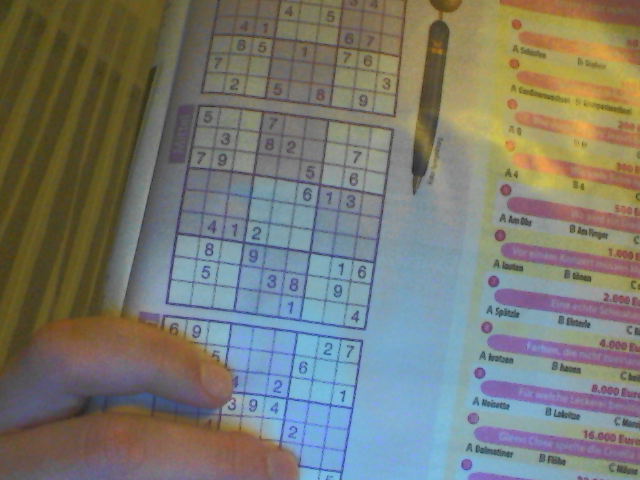
\includegraphics[width=\textwidth]{imgs/unwarp_frame.png}
        \caption{Original frame.}
    \end{subfigure}

    \begin{subfigure}[b]{0.70\textwidth}
        \centering
        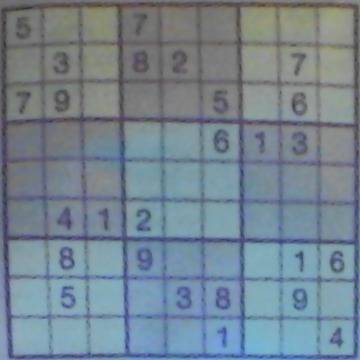
\includegraphics[width=\textwidth]{imgs/unwarp.png}
        \caption{Output of the canny filter.}
    \end{subfigure}
    \caption{Unwarped sudoku field.}
    \label{fig:unwarping}
\end{figure}

\subsection{Digit Segmentation}

Now that the image of the sudoku field is present without distortion at a
fixed size we can apply a grid to it to roughly divide it into the single
cells. In each cell we have to decide if it contains a digit and segment
it, respectively.

The segmentation of the digits is illustrated in figure \ref{fig:digit_seg}.
The coarse segmentation is done by applying a gaussian blur to remove some
noise followed by an adaptive thresholding
\footnote{\url{http://docs.opencv.org/modules/imgproc/doc/miscellaneous_transformations.html\#adaptivethreshold}}. 
In contrast to an ordinary threshold, the threshold value varies locally
depending on the mean value of the pixel intensities in the 
neighborhood around the pixel.

\begin{figure}
  \centering
  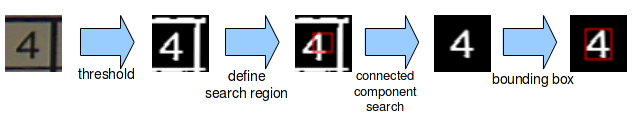
\includegraphics[width=0.9\textwidth]{imgs/segmentation.png}
  \caption{Digit segmentation process.}
  \label{fig:digit_seg}
\end{figure}

Although this operation works pretty well there is often the problem that
parts of the grid lines lie inside the image of the cell. Since these lines
have approximately the same thickness as the digits they can not be removed
by the thresholding. To overcome this issue we assume that a small region
in the middle of the image does only contain pixels belonging to the digit.
Starting from these pixels we start a a connected component search to find the
rest of the digit. All other pixels will be discarded.

\subsection{Digit Classification}

In order to be able to find a solution of the sudoku we must classify the
found digits. First, we were thinking of using an existing OCR framework
for this task. Finally we decided to build our own classifier to have more influence
on the classification.

We evaluated three different types of classifiers for this task: \emph{K-Nearest Neighbor},
\emph{Support Vector Machine} and a \emph{Neural Network}. Each of them can be enabled
during compilation of the application. We have chosen to use the Support Vector Machine
since it yielded the best results. In section \ref{sec:results} we will discuss the performance
of them in detail.

Although there would be the possibility to compute descriptors of the segmented digits
(eg. Histogram of Oriented Gradients) we decided to use the plain binary image data
as input to the classifier.

The only preprocessing steps for the training and classification are:

\begin{description}
  \item[Deskewing:] This operation makes the classification more robust for different
  fonts and for handwritten digits in future. This is done by calculating the central
  moments of the pixels. The skewness is given by the third central moments, which is
  used to construct a affine transformation matrix for deskewing.
  \item[Crop:] Since there is a lot of unimportant background in the digit images, we
  crop the image to only include as much background as required. This is done by finding
  the bounding box of the digit contour.
  \item[Rescale:] The support vector machine requires all training and test data to have
  the same dimensionality. After cropping the image, there is no guarantee, that all resulting
  images will have the same size. We overcome this issue by simply rescaling all input
  images for the Support Vector Machine to size $16 \times 16$. Therefore, every input
  vector has 256 dimensions.
  \item[Principal Component Analysis (PCA):] All of the three classificators are able to
  perform a PCA prior to the training (and consequently, also prior to the classification).
  However, at this time there is no possibility to save and load the PCA, respectively.
  So this feature is disabled by default. 
\end{description}

\subsubsection{Training data}

The training data for the classificator can be extracted directly from the application. It
provides a gui, which provides the user with a possibility to label the training images
by hand. The application is then able to save the extracted training data to the file system.
The file system structure reflect the labeling. Figure \ref{fig:extract_dlg} shows how the
labeling mechanism works.

\subsection{Sudoku Solving}

\subsection{Presenting the Solution}

The projection of the solution onto the original image is not a big deal, since we already
found the homography as described in section \ref{sec:find}. Therefore we can draw the solution
on the rectified imaged and apply the homography inversely.

%%%%%%%%%%%%%%%%%%%%%%%%%%%%%
\section{Implementation}
%%%%%%%%%%%%%%%%%%%%%%%%%%%%%

The application was developed using OpenCV and Qt. No further libraries were used.

The most important parameters of the implementation can be found in \emph{include/settings.hpp}.
Since these parameters are tweaked to be best for the test system, it may be necessary to
adjust them if you are trying to run the application on other webcams. 

%%%%%%%%%%%%%%%%%%%%%%%%%%%%%
\section{Evaluation/Results}
%%%%%%%%%%%%%%%%%%%%%%%%%%%%%
\label{sec:results}

\subsection{Field Extraction}

In most cases, the field extraction works very well. The performance of it highly depends on the 
parameters \emph{CANNY\_LOW} and \emph{CANNY\_HIGH}. Currently, they are tweaked to yield the best
results for the images delivered by the webcam of the test system.

However, the application is currently not able to distinguish between contours of sudoku fields and
contours of other objects. The only assumptions that were made are:

\begin{itemize}
  \item The sudoku field is the most prominent object in the image, therefore the biggest contour
  belongs to the sudoku.
  \item The contour needs to be convex, so all non-convex contours are discarded.
\end{itemize}

If those properties are given within the image, the segmentation of the sudoku field works very well. 

If the motion of the sudoku field in the video is very high, there will be no closed contour of it,
and therefore, the contour will not be recognized. However, the application does not reset everything because
the sudoku was not found in one frame. Instead it waits for 10 frames to decide wether the sudoku is gone
or not.

\subsection{Digit Segmentation}
\label{sec:class_perf}

Since the segmentation of the digits was kept very simple, there are not many things that could go
wrong. For all our tested sudoku sheets the segmentation worked very well. However, there could
be problems, if the font of the digits is very thin. In this case, the adaptive threshold could
possibly removes the digit, but we did not find a sudoku with such a font.

\subsection{Classification}

The classification performance can be measured in many different ways. We have chosen to test the
performance using k-fold-cross validation with $k=10$. Table \ref{tab:class_perf} shows the results
for the three different classificators.

\begin{table}
    \centering
    \begin{tabular}{|l|l|}
    \hline
    \textbf{Classificator}          & \textbf{Hit rate}   \\ \hline
    k-nearest Neighbors    & $ 99.243\%$ \\ \hline
    Support Vector Machine & $ 98.481\%$    \\ \hline
    Neural Network         & $ 60.521\%$    \\ \hline
    \end{tabular}
    \caption{Performance of the different classificators.}
    \label{tab:class_perf}
\end{table}

The Support Vector Machine and k-nearest Neighbors are very similar with respect to the classification
performance. Anyway, the SVM is a little bit better so it was chosen to be the default configuration.

The Neural Network showed a really bad performance. This is mainly because we did not find good training
parameters for it. Since the training of a nerual network is a long running process and the other 
classificators performed very well, we did not investigate this further. The presented hit rate was
achieved with one hidden layer of $35$ neurons.

\subsubsection{Performance on new Sudoku Fields}

In section \ref{sec:class_perf} the performance on the training set itself was shown but the application
should work with any sudoku. We did not really evaluate this but subjectively we can say, that most
sudokus work out of the box. This is no surprise, because most of the sudokus use a similar fonts with
similar scaling.

\subsection{Sudoku Solver}

%%%%%%%%%%%%%%%%%%%%%%%%%%%%%
\section{Discussion}
%%%%%%%%%%%%%%%%%%%%%%%%%%%%%

Blablabla

%%%
%%% end main document
%%%
%%%%%%%%%%%%%%%%%%%%%%%%%%%%%%%%%%%%%%%%%%%%%%%%%%%%%%%%%%%%%%%%%%%%%%%%%%%%%%%%

% \appendix  %% include it, if something (bibliography, index, ...) follows below

%%%%%%%%%%%%%%%%%%%%%%%%%%%%%%%%%%%%%%%%%%%%%%%%%%%%%%%%%%%%%%%%%%%%%%%%%%%%%%%%
%%%
%%% bibliography
%%%
%%% available styles: abbrv, acm, alpha, apalike, ieeetr, plain, siam, unsrt
%%%
% \bibliographystyle{plain}

%%% name of the bibliography file without .bib
%%% e.g.: literatur.bib -> \bibliography{literatur}
% \bibliography{literature}

\end{document}
%%% }}}
%%% END OF FILE
%%%%%%%%%%%%%%%%%%%%%%%%%%%%%%%%%%%%%%%%%%%%%%%%%%%%%%%%%%%%%%%%%%%%%%%%%%%%%%%%
%%% Notice!
%%% This file uses the outline-mode of emacs and the foldmethod of Vim.
%%% Press 'zi' to unfold the file in Vim.
%%% See ':help folding' for more information.
%%%%%%%%%%%%%%%%%%%%%%%%%%%%%%%%%%%%%%%%%%%%%%%%%%%%%%%%%%%%%%%%%%%%%%%%%%%%%%%%
%% Local Variables:
%% mode: outline-minor
%% OPToutline-regexp: "%% .*"
%% OPTeval: (hide-body)
%% emerge-set-combine-versions-template: "%a\n%b\n"
%% End:
%% vim:foldmethod=marker